\section{Wartości bezwzględne na ciele}
Celem \prawo{Gouvea\\2} tego rozdziału jest wyłożenie solidnych podstaw, na których później zbudujemy bardziej szałową teorię.
Najpierw zastanowimy się, jakie cechy powinna mieć wartość bezwzględna, by móc ją zdefiniować dla dowolnego ciała.
Następnie przekonamy się, co jesteśmy w stanie zrobić, kiedy umiemy już mierzyć odległości.
Aż do końca książki przez $\R_+$ oznaczamy zbiór $\{x \in \R : x \ge 0\}$, zaś $\cialo$ będzie bliżej nieokreślonym ciałem.

\begin{definicja}
	\emph{Wartość bezwzględna} \prawo{Gouvea\\2.1} to funkcja $\|\cdot\| \colon \cialo \to \R_+$, że $\|x\| = 0$ tylko dla $x = 0$, dla wszystkich $x, y \in \cialo $ zachodzi $\|xy\| = \|x\| \cdot \|y\|$ oraz $\|x + y\| \le \|x\| + \|y\|$.
	
	Wartość bezwzględną spełniającą nieco mocniejsze oszacowanie $\|x+y\| \le \max \{\|x\|, \|y\|\}$ będziemy określać niearchimedesową.
\end{definicja}

Nie jest jeszcze do końca jasne, czy obiekt o postulowanych własnościach w ogóle istnieje, jednak wkrótce przekonamy się o tym na bardzo konkretnym przykładzie.
Ciała, w których spełniona jest ostatnia nierówność nazywa się na jej cześć ultrametrycznymi.
To głównie nimi będziemy zainteresowani.

Przykładem wartości bezwzględnej na $\cialo = \Q$, $\R$ jest funkcja określona w następujący sposób.
Jeśli $x \ge 0$, to kładziemy $|x| := x$, w przeciwnym razie niech $|x| := -x$.
Łatwo sprawdzić, że można ją przedłużyć do ciała liczb zespolonych wzorem $|a + bj| = (a^2+b^2)^{1:2}$.
Przyjmując $x = y = 1$ widzimy, że nie jest ona niearchimedesowa.
Z pewnych przyczyn oznaczamy ją przez $|\,\,|_\infty$.

Swoją drogą, litera $j$ zawsze służyć będzie za symbol jednostki urojonej, czyli pierwiastka równania $x^2 + 1 = 0$ i nigdy nie pojawi się jako indeks sumowania.

Na każdym ciele mamy prawo zdefiniować najnudniejszą ze wszystkich możliwych wartości bezwzględnych przez określenie $|x| = 1$, wtedy i tylko wtedy gdy $x \neq 0$ oraz $|0| = 0$.
Jest wprawdzie niearchimedesowa, jednak często będzie pomijana w twierdzeniach.

Pojęć ,,wartość bezwzględna'' oraz ,,norma'' można używać zamiennie, a przy tym to drugie jest znacznie krótsze.

\begin{fakt}
	Na skończonym ciele istnieje tylko trywialna norma.
\end{fakt}

\begin{proof}
	Wynika to z twierdzenia Lagrange'a dla $\cialo^\times$.
\end{proof}

Wszystkie ciekawe ciała (z normami) są więc nieskończone.
Należy zwrócić uwagę na to, że choć $\mathbb F_p$ (ciało o $p$ elementach) jest dla nas mało atrakcyjne, to nie rozumiemy jeszcze jego (być może nieskończonych!) rozszerzeń.

\begin{definicja}
	Funkcja $v_p \colon \Z \setminus \{0\} \to \R$, ,,największy wykładnik $v$, że $p^v$ dzieli argument'', to waluacja $p$-adyczna (krotność $p$ w rozkładzie na czynniki pierwsze).
\end{definicja}

Łatwo sprawdzić, że funkcja $v_p$ jest dobrze określona i przedłuża się w jednoznaczny sposób do ciała liczb wymiernych: dla $\frac x y \in \Q^\times$ piszemy $v_p(\frac xy) = v_p(x) - v_p(y)$.

Powszechnie przyjmuje się, że $v_p(0) = \infty$, ponieważ zero można dzielić dowolnie wiele razy przez $p$.

\begin{przyklad}
	$v_5(400) = v_5(5^2 \cdot 16) = 2$.
	$v_3(\frac{123}{48}) = v_3(3^1 \cdot 41) - v_3(3^1 \cdot 16) = 0$.
\end{przyklad}

Waluacja ma dwie bardzo ważne własności determinujące geometrię liczb $p$-adycznych.
Ich znaczenie docenimy dwa fakty dalej.

\begin{lemat} \label{diewildenjahre}
	Niech $x, y \in \Q$.
	Wtedy $v_p(xy) = v_p(x) + v_p(y)$ i $v_p(x+y) \ge \min \{v_p(x), v_p(y)\}$ ze stosowną umową dla $v_p(0) = \infty$.
\end{lemat}

Nadszedł czas na raczej nieoczekiwaną sztuczkę.
Druga własnosć z lematu przypomina nieco warunek, jaki musi spełniać norma, by zasłużyć na przydomek niearchimedesowej.
Produkt z lematu zmienia się w sumę (jak przy nakładaniu logarytmu), zaś sama nierówność zmieniła kierunek.
Cofniemy to funkcją wykładniczą i odwróceniem znaków.

\begin{fakt}
	Funkcja $|x|_p = p^{-v_p(x)}$ (dla $x \neq 0$), $|0|_p = 0$ to niearchimedesowa norma na $\Q$.
\end{fakt}

\begin{proof}
	Oczywisty, jeśli podaliśmy dowód wcześniejszego lematu.
\end{proof}

Dla przykładu, $|3/686|_7 = 7^2 = 49$, ale $|177553|_7 = 1$.
Normy $p$-adyczne nie mierzą więc odległości od zera, ale stopień podzielności.

\begin{fakt}
	Jeśli $\pierscien$ jest dziedziną całkowitości z ciałem ułamków $\cialo$, zaś $v \colon \pierscien \setminus \{0\} \to \R$ waluacją (funkcją, dla której prawdziwy jest lemat \ref{diewildenjahre}) przedłużoną do całego $\cialo$ wzorem $v(\frac xy) = v(x)-v(y)$, to funkcja $\cialo \to \R_+$, $\|z\|_v = \exp(-v(z))$ i $\|0\| = 0$ jest niearchimedesową normą.

	Odwrotnie, gdy $\|\cdot\|$ jest niearchimedesową normą, to $-\log \|\cdot\|$ jest waluacją.
\end{fakt}

Dowód pomijamy, albowiem nie różni się znacząco od tego, który już przeprowadziliśmy.
Wymaga jedynie uważnego przeczytania definicji ciała ułamków.
Zauważmy, że fakt jest prawdziwy niezależnie od podstawy funkcji wykładniczej (logarytmu), choć pewne wybory są lepsze od innych.
Zrozumiemy to po zdefiniowaniu pierścienia adeli.

Literą $\pierscien$ oznaczać będziemy różnej maści pierścienie, zazwyczaj przemienne.

Zdefiniujemy teraz jeszcze dwie normy na ciele funkcji wymiernych $\cialo(t)$.
Jedną z nich jest stopień: $v_\infty(f) = \deg f$, określony na pierścieniu $\cialo[t]$ i stosownie przedłużony.

Druga z nich jest wyrafinowana.
Niech wielomian $p(t) \in \cialo[t]$ będzie nierozkładalny.
W pierścieniu $\cialo[t]$ rozkład jest jednoznaczny, zatem poniższa definicja ma ręce i nogi:

\begin{definicja}
	Dla wielomianu $f(t) \in \cialo[t]$ niech $v_{p(t)}(f(t))$ będzie krotnością, z jaką czynnik $p(t)$ występuje w rozkładzie $f(t)$.
\end{definicja}

Ciało $\cialo(t)$ zawiera podpierścień $\cialo[1/t]$, w którym ,,wielomian'' $1/t$ jest nierozkładalny.
Okazuje się, że $v_{1/t} = v_\infty$, zatem wszystkie nasze normy są ,,$p(t)$''-adycznego typu.

\begin{fakt}
	Norma \prawo{Gouvea\\2.2} $\|\cdot\|$ na ciele $\cialo$ jest niearchimedesowa, wtedy i tylko wtedy, gdy $\|n\| \le 1$ dla każdego $n \in \Z$ (włożonego w $\cialo$).
\end{fakt}

\begin{proof}
	Oczywista równość $\|\pm 1\| = 1$ pociąga $\|n \pm 1\| \le \max \{\|n\|, 1\}$.	
	Skorzystanie z dobrodziejstw indukcji matematycznej kończy dowód w prawo.

	W lewą stronę wymagane są już czary-mary.
	Ponieważ $\|x + y\| \le \max \{\|x\|, \|y\|\}$ jest oczywistą nierównością dla $y = 0$, pokażemy $\|z+1\| \le \max \{\|z\|, 1\}$ (dla $z \in \cialo$).
	Niech $m$ będzie liczbą naturalną.
	Wtedy
	\[
		\|z+1\|^m 
		=   \left\|\sum_{i=0}^m {m \choose i} z^i \right\| 
		\le \sum_{i=0}^m \left\|{m \choose i} z^i \right\| 
		\le \sum_{i=0}^m \|z\|^i
		\le (m+1) \max \{1, \|z\|^m\}.
	\]

	Pierwiastkujemy obie strony i przechodzimy z $m$ do nieskończoności.
\end{proof}

Własność Archimedesa mówi, że $\sup\{|n| : n \in \Z\} = \infty$.
Jeżeli supremum okaże się być skończone, to wynosi $1$ i wartość nie jest archimedesowa.
Innych możliwości nie ma.

\begin{historia}[Archimedes z Syrakuz]\end{historia}

\section{Fałszywa geometria}
Ciało, gdzie wszystkie działania są ciągłe, nazywa się ciałem topologicznym, takie może być ciało z metryką.
Przestrzenie z taką nierównością wydają się być dziwaczne i rzeczywiście nimi są.
Skoro pomiar odległości nie należy do normalnych, to i geometria będzie nie z tej Ziemi.

\begin{fakt}
	W \prawo{Gouvea\\2.3} niearchimedesowym ciele $\cialo$, $\|x\| \neq \|y\|$ pociąga $\|x+y\| = \max \{\|x\|, \|y\|\}$.
\end{fakt}

\begin{proof}
	$\|x\| > \|y\|$ pociąga pierwszą nierówność, $\|x+y\| \le \|x\| = \max\{\|x\|,\|y\|\}$.

	Ale $x = x+y-y$, więc $\|x\| \le \max \{\|x+y\|, \|y\|\}$.
	Nierówność zachodzi tylko wtedy, gdy $\max\{\|x+y\|, \|y\|\} = \|x+y\|$.
	To daje drugą nierówność $\|x\| \le \|x+y\|$.
\end{proof}

Używanie niearchimedesowych norm jest jak mierzenie odległości do gwiazd z innej galaktyki.
Innymi słowy, wszystkie trójkąty są równoramienne, a ich ramiona są dłuższe od podstaw.
Zbadamy jeszcze kule.
Uwaga. 
Nie zawsze domknięciem kuli otwartej jest kula domknięta o tym samym promieniu.
Z tego względu stosować będziemy zapis $\kula(x, r)$ (kula otwarta) oraz $\kula[x, r]$ (domknięta).

\begin{fakt}
	W niearchimedesowym ciele $\cialo$ każdy punkt kuli (otwartej, domkniętej) jest jej środkiem.
	Jeśli $r > 0$, to kula jest otwarnięta.
	Dwie kule (domknięte, otwarte) są rozłączne lub zawarte jedna w drugiej.
\end{fakt}

\begin{proof}
	Wszystko jest proste, tylko nic nie jest oczywiste.
	\begin{enumx}
		\item Jeśli $y \in \kula(x, r)$, to $\|x-y\| < r$.
		Biorąc dowolny $z$, że $\|z-x\| < r$, dostajemy $\|z-y\| < r$ (niearchimedesowo), zatem $\kula(x,r) \subseteq \kula(y,r)$.
		Podobnie w drugą stronę.
		\item Każda otwarta kula jest otwartym zbiorem.
		Weźmy $y$ z brzegu $\kula(x,R)$, do tego $r \le R$.
		Wtedy pewien $z$ jest w $\kula(x,R) \cap \kula(y,r)$ (przekrój jest niepusty).
		To oznacza, że $\|z-x\| < R$ oraz $\|z - y\| < r \le R$, więc $\|x-y\| \le R$ i $y \in \kula(x,R)$.
		\item Weźmy nierozłączne $\kula(x,r)$, $\kula(y,R)$, że $r \le R$.
		Wtedy pewien $z$ leży w obydwu kulach.
		Ale $\kula(x,r) = \kula(z,r)$ zawiera się w $\kula(z,R) = \kula(y,R)$. \qedhere
	\end{enumx}
\end{proof}

Analogiczne rozumowanie można przeprowadzić dla kul domkniętych.

Efektem ubocznym jest to, że gdy $\cialo = \Q$, zaś $\|\cdot\| = |\cdot|_p$, to domknięte kula $\kula [0,1]$ jest sumą rozłączną otwartych $\kula (i, 1)$ dla $0 \le i < p$.
,,Sfera'' ($\{x \in \cialo : \|x-y\| = r\}$) jest otwarnięta (i \emph{nie jest} brzegiem kuli).

Nietrywialne otwarte kule niczym nie różnią się od swoich domkniętych koleżanek.
To pokazuje, do jak wielu fałszywych wniosków można dojść myśląc o każdej przestrzeni metrycznych jak o $\R^n$.

Cassels nazywa nasze normy waluacjami, a przy tym upiera się przy innej nierówności:
$\|x+y\| \le C \max \{\|x\|, \|y\|\}$.
Na stałą $C = 2$ można sobie pozwolić zawsze (zmieniając normę, ale nie topologię) i dostać nierówność trójkąta, na $C= 1$ (ultra) już niekoniecznie.

Wygląda na to, że nigdy nie będzie zgody w sprawie nomenklatury.

\begin{Figure}
 \centering
 \frame{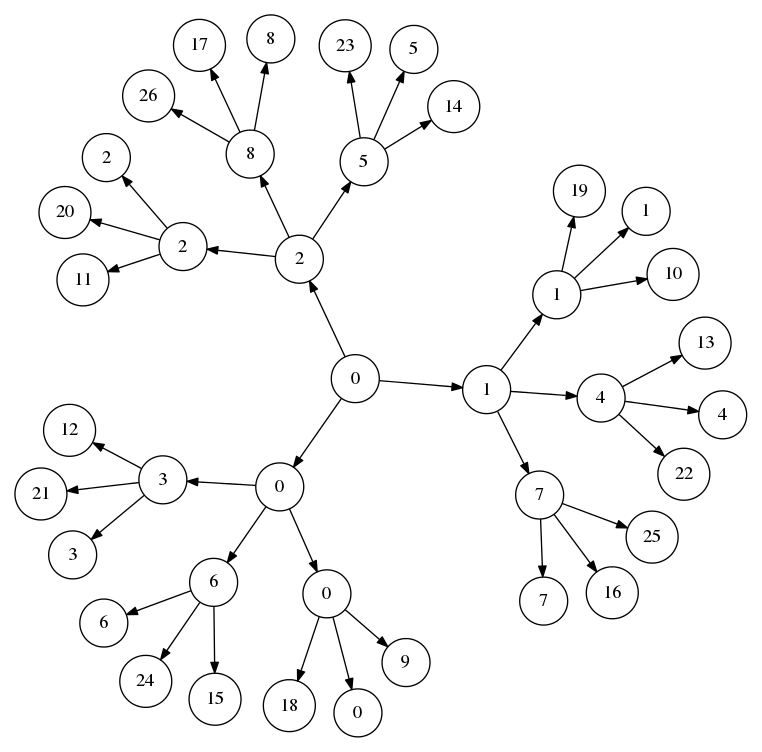
\includegraphics[width=0.85\linewidth]{images/drzewo.png}}
 \captionof{figure}{Rzekomo jest to drzewiasta struktura (niezbudowanego jeszcze) $\Z_3$.}
\end{Figure}

%%% skompilowane przez neato
% digraph G {
%     nodesep=0.3;
%     ranksep=0.2;
%     margin=0.1;
%     node [shape=circle];
%     edge [arrowsize=0.8];
% 	ae [label="0"]; 
% 	aq [label="0"]; 
% 	ar [label="1"]; 
% 	aw [label="2"]; 
% 	de [label="0"];
% 	dq [label="3"];
% 	dr [label="6"];
% 	dw [label="1"];
% 	ee [label="4"];
% 	eq [label="7"];
% 	er [label="2"];
% 	ew [label="5"];
% 	fe [label="8"];
% 	fq [label="0"];
% 	fr [label="9"];
% 	fw [label="18"];
% 	ge [label="3"];
% 	gq [label="12"];
% 	gr [label="21"];
% 	gw [label="6"];
% 	qe [label="15"];
% 	qq [label="24"];
% 	qr [label="1"];
% 	qw [label="10"];
% 	re [label="19"];
% 	rq [label="4"];
% 	rr [label="13"];
% 	rw [label="22"];
% 	se [label="7"];
% 	sq [label="16"];
% 	sr [label="25"];
% 	sw [label="2"];
% 	te [label="11"];
% 	tq [label="20"];
% 	tr [label="5"];
% 	tw [label="14"];
% 	we [label="23"];
% 	wq [label="8"];
% 	wr [label="17"];
% 	ww [label="26"];
% 	de -> fq;
% 	de -> fr;
% 	de -> fw;
% 	dq -> ge;
% 	dq -> gq;
% 	dq -> gr;
% 	dr -> gw;
% 	dr -> qe;
% 	dr -> qq;
% 	dw -> qr;
% 	dw -> qw;
% 	dw -> re;
% 	ee -> rq;
% 	ee -> rr;
% 	ee -> rw;
% 	eq -> se;
% 	eq -> sq;
% 	eq -> sr;
% 	er -> sw;
% 	er -> te;
% 	er -> tq;
% 	ew -> tr;
% 	ew -> tw;
% 	ew -> we;
% 	fe -> wq;
% 	fe -> wr;
% 	fe -> ww;
%     ae -> aq;
%     ae -> ar;
%     ae -> aw;
%     aq -> de;
%     aq -> dq;
%     aq -> dr;
%     ar -> dw;
%     ar -> ee;
%     ar -> eq;
%     aw -> er;
%     aw -> ew;
%     aw -> fe;
% }

